\documentclass[11pt, a4paper]{article}
\usepackage[utf8]{inputenc}
\usepackage{fancyhdr}
\usepackage{graphicx}
\PassOptionsToPackage{hyphens}{url}\usepackage{hyperref}
\usepackage{geometry}
\usepackage[
backend=biber,
style=apa,
]{biblatex}
\usepackage{kotex}

\addbibresource{reference.bib}

\pagestyle{fancy}
\fancyhf{}
\setlength{\headheight}{14pt}
\rhead{Master dissertation}
\lhead{sukhoon park}
\cfoot{\thepage}

\begin{document}

\title{AI Report}
\author{Siyun Min}
\maketitle

\tableofcontents

\section{중산층 개념 논의}
중산층 관련 발표를 하는걸로. 지도교수 컨펌 필요. 이론적으로 쓰고 그걸 학위논문화시키고 다시 요약본과 분석을 논문으로 재생산하는 것.
\subsection{한국에서의 중산층이란?}

\subsection{중민이론, 한상진, 김홍중}

\subsection{해외 중산층 논의}

\section{한국적인 상황}

\subsection{위험사회, 위험 바라보는 두 가지 시각들}

\subsection{학자 정리. 이재열, 홍두승, 장경섭.}

\subsection{장경섭에서 부모 부양이라는 것을 끄집어 내는 것.}

\section{국민이전계정}
\subsection{통계청 발표 자료 참고+Manual(확보완료)}
\subsection{데이터 요청해서 받고 기초분석. 지역별로? RDC}

\section{실제분석}
\subsection{네트워크?}
\subsection{들어간 기초자료}
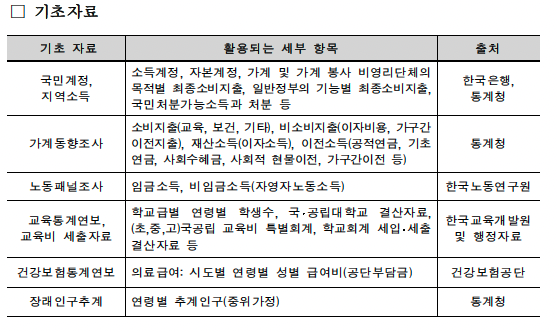
\includegraphics[]{basic_material_list.png}



\printbibliography

\end{document}